% Uncomment for handout
\def\HANDOUT{}


\ifdefined\HANDOUT
\documentclass[handout]{beamer}
\usepackage{pgfpages}
\pgfpagesuselayout{4 on 1}[letterpaper,landscape,border shrink=5mm]
\else
\documentclass{beamer}
\fi

\mode<presentation>
{
  \usetheme{Warsaw}
  \definecolor{sered}{rgb}{0.78, 0.06, 0.18}
  \definecolor{richblack}{rgb}{0.0, 0.0, 0.0}
  \setbeamercolor{structure}{fg=sered,bg=richblack}
  %\setbeamercovered{transparent}
}


\usepackage[english]{babel}
\usepackage[latin1]{inputenc}
\usepackage{times}
\usepackage[T1]{fontenc}
\usepackage{tikz}
\usepackage{graphicx}
\usepackage[export]{adjustbox}
\usepackage{fancyvrb}
\usepackage{amsmath}
\usepackage{amssymb}
\usepackage{esvect}

\makeatletter
\newcommand{\imagesource}[1]{{\centering\hfill\break\hbox{\scriptsize Image Source:\thinspace{\tiny\itshape #1}}\par}}
\newcommand{\image}[3][\@nil]{%
        \def\tmp{#1}%
        \begin{center}
        \ifx\tmp\@nnil
            \includegraphics[max height = 0.55\textheight, max width = \textwidth]{images/#2}
        \else
            \includegraphics[max height = 0.50\textheight, max width = \textwidth]{images/#2}
            \linebreak
            #1
        \fi
        \linebreak
        {\tiny Image Source:\thinspace{\tiny #3}}
        \end{center}
}

\newenvironment{code}{%
 \VerbatimEnvironment
 \begin{adjustbox}{max width=\textwidth, max height=0.7\textheight}
 \begin{BVerbatim}
  }{
  \end{BVerbatim}
 \end{adjustbox}
}

\title{05 - PCA - Principal Component Analysis}


\author{Robert Lowe}

\institute[Southeast Missouri State University] % (optional, but mostly needed)
{
  Department of Computer Science\\
  Southeast Missouri State University
}

\date[]{}
\subject{}

\pgfdeclareimage[height=1.0cm]{university-logo}{images/semo-logo}
\logo{\pgfuseimage{university-logo}}



\AtBeginSection[]
{
  \begin{frame}<beamer>{Outline}
    \tableofcontents[currentsection]
  \end{frame}
}


\begin{document}

\begin{frame}
  \titlepage
\end{frame}

\begin{frame}{Outline}
  \tableofcontents
\end{frame}


% Structuring a talk is a difficult task and the following structure
% may not be suitable. Here are some rules that apply for this
% solution: 

% - Exactly two or three sections (other than the summary).
% - At *most* three subsections per section.
% - Talk about 30s to 2min per frame. So there should be between about
%   15 and 30 frames, all told.

% - A conference audience is likely to know very little of what you
%   are going to talk about. So *simplify*!
% - In a 20min talk, getting the main ideas across is hard
%   enough. Leave out details, even if it means being less precise than
%   you think necessary.
% - If you omit details that are vital to the proof/implementation,
%   just say so once. Everybody will be happy with that.

\section{PCA}

\begin{frame}{History}
    \begin{columns}
    \column{0.5\textwidth}
    \begin{itemize}
        \item Invented in 1901 by Karl Pearson
        \item Analogous to the Principal Axis Theorem
    \end{itemize}
    \column{0.5\textwidth}
    \image[\textbf{Karl Pearson}\linebreak{\scriptsize 1857-1936}]{Pearson}{\href{https://en.wikipedia.org/wiki/Karl_Pearson}{Wikipedia}}
    \end{columns}    
\end{frame}

\begin{frame}{Principal Component Analysis}
    \begin{itemize}
        \item Given an $m\times n$ matrix $X$ where each row is a feature vector.
        \item Compute a matrix $T$ by changing the basis of $X$:
        \[
        T = XW
        \]
        \item $W$ is a $n\times n$ matrix, where each column is a basis vector.
        \item $W$ is computed as:
        \[
        T = eigen(X^TX)
        \]
    \end{itemize}
\end{frame}

\begin{frame}{The PCA Space}
    \begin{itemize}
        \item Each column of $W$ is a principal component of $X$.
        \item $W$ is ordered according to how much variance it captures.
        \item Projecting $X$ onto a subset of $W$ will capture some, but not all, of the variance of $X$.
        \item Sometimes that is good enough! We can reduce dimensions this way!
        \item Each component represents a linear mixture of all measurements in the feature vector.
    \end{itemize}
\end{frame}

\section{Eigenpets}

\begin{frame}{Eigenpets}
    \begin{itemize}
        \item 160 pictures, 80 of cats, 80 of dogs.
        \item Each picture is 64 pixels wide and 64 pixels tall.
        \item The data are represented as gray scale values in the range $[0, 255]$.
        \item In the data set, each column is an image. 
        \item The feature space has $4096$ variables!
        \item Luckily, not all of them are likely to be important.
    \end{itemize}
\end{frame}

\begin{frame}[fragile]{Data Set and Starter Code}
    \begin{code}
import pandas as pd
import matplotlib.pyplot as plt
import numpy as np
import seaborn as sns
from PIL import Image
# import your pca function here

def showPets(data, title="", labels=[]):
    '''
    Show a plot of an eigenpet.
    data is a numpy array with pet images in each column
    '''
    # function omitted to save space on the slide
    # it's all in canvas if you want to see the full text!

# get the cats and dogs
cats = pd.read_csv("cat.csv", header=None)
dogs = pd.read_csv("dog.csv", header=None)
pets = np.hstack((cats, dogs))

# Show two cats, and two dogs
showPets(np.hstack((pets[:, 0:1], pets[:, 40:41], pets[:, 80:81], pets[:, 120:121])), 
         "Sample Pets", ("Cat 1", "Cat 40", "Dog 1", "Dog 40"))

    \end{code}
\end{frame}

\begin{frame}{Sample Pets}
    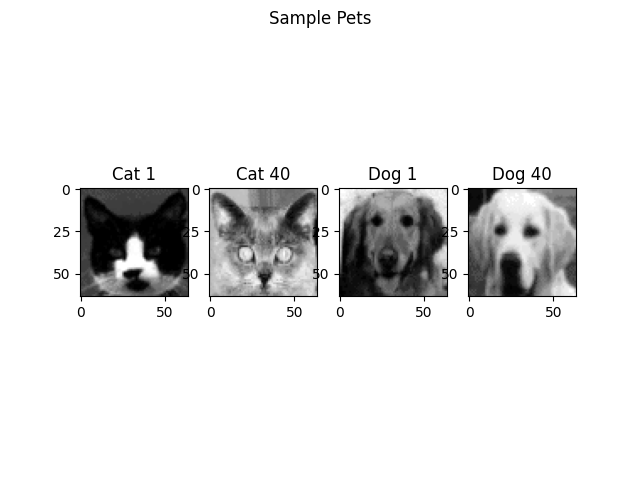
\includegraphics[height=0.9\textheight]{images/eigenpets-sample}
\end{frame}

\begin{frame}[fragile]{Compute the Average Pet}
    \begin{code}
# compute the "average" pet
avgPet = pets.mean(axis=1, keepdims=True)
avgCat = pets[:, 0:80].mean(axis=1, keepdims=True)
avgDog = pets[:, 80:160].mean(axis=1, keepdims=True)
showPets(np.hstack((avgPet, avgCat, avgDog)), 
         "Average Pets", ["Pet", "Cat", "Dog"])
    \end{code}
\end{frame}

\begin{frame}{Compute the Average Pet}
    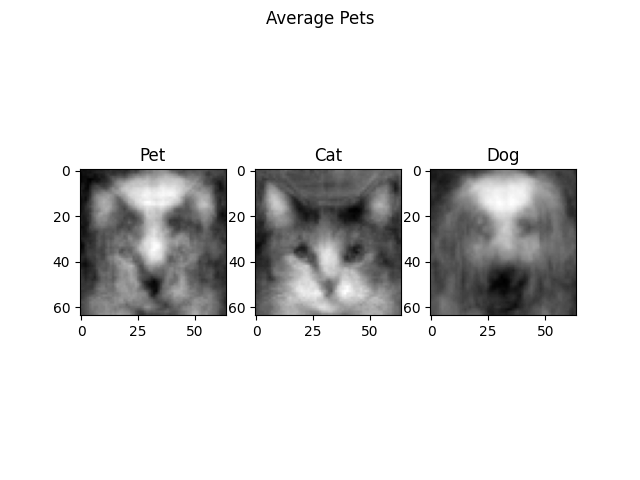
\includegraphics[height=0.9\textheight]{images/eigenpets-average}
\end{frame}

\begin{frame}[fragile]{Run PCA on the Pets}
    \begin{code}
# run pca on the pets
evect, evals, varexp, cumvarexp = pca(pets.T)

# get rid of any imaginary components
evect = np.real(evect)
evals = np.real(evals)
varexp = np.real(varexp)
cumvarexp = np.real(cumvarexp)


#show the first few components
showPets(evect[:, 0:6], "First 6 Principal Components")
    \end{code}
\end{frame}

\begin{frame}{Run PCA on the Pets}
    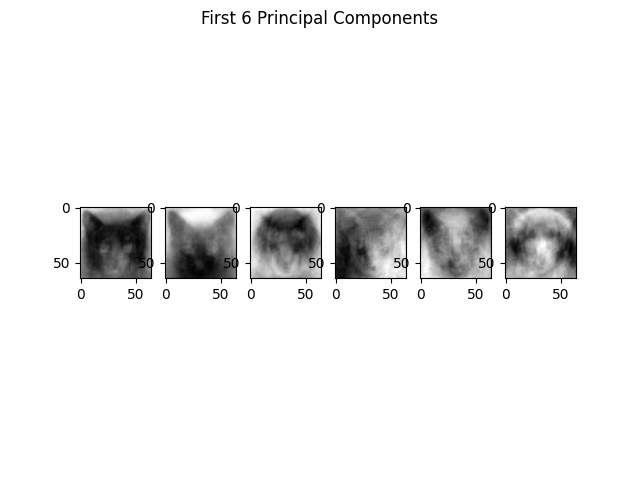
\includegraphics[height=0.9\textheight]{images/eigenpets-components}
\end{frame}

\begin{frame}[fragile]{Elbow Plot}
\begin{code}
#show the elbow plot of the components
plt.title("Elbow Plot of Principal Components")
sns.lineplot(x=range(1, len(cumvarexp)+1), y=cumvarexp)
plt.show()
\end{code}
\end{frame}

\begin{frame}{Elbow Plot}
    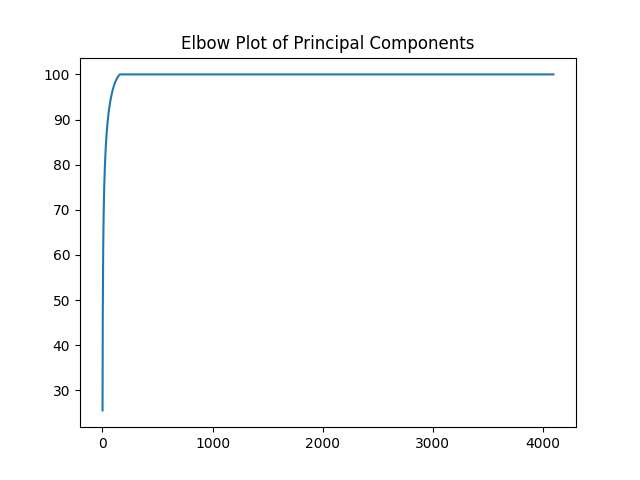
\includegraphics[height=0.9\textheight]{images/eigenpets-elbow}
\end{frame}

\begin{frame}{Elbow Plot}
    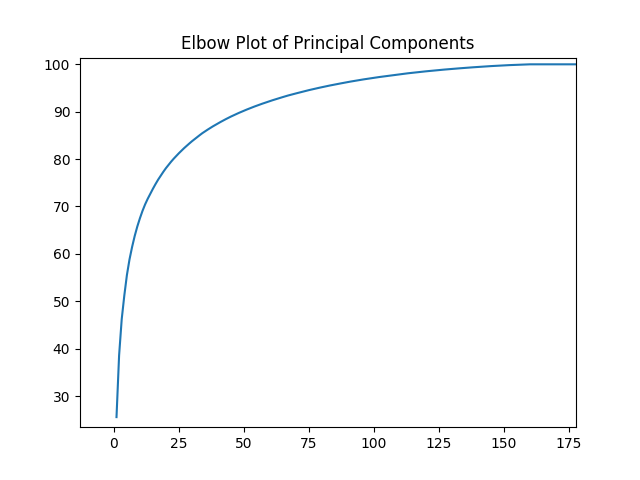
\includegraphics[height=0.9\textheight]{images/eigenpets-elbow-zoomed}
\end{frame}

\end{document}
